
\begin{figure}


	\centering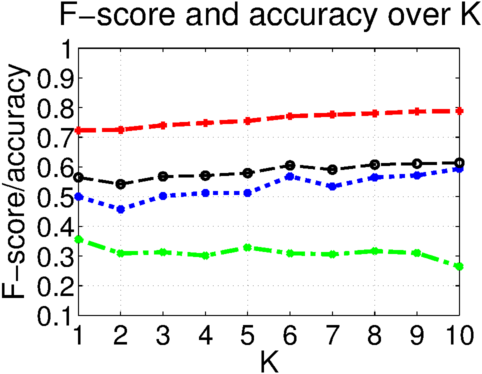
\includegraphics[width=0.3\textwidth]{tex/appendices/test/sflux2010FP.png}
	\centering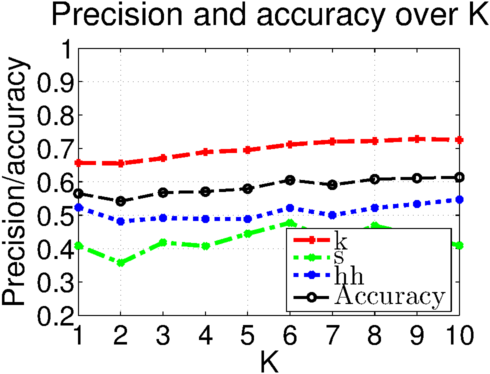
\includegraphics[width=0.3\textwidth]{tex/appendices/test/sflux2010_P.png}
	\centering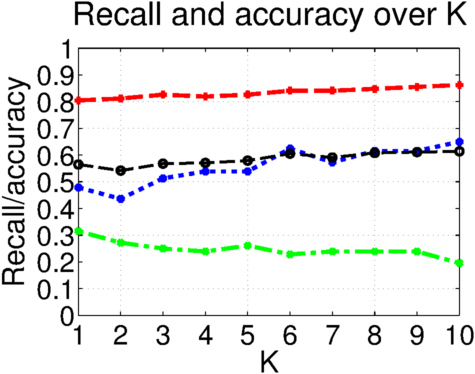
\includegraphics[width=0.3\textwidth]{tex/appendices/test/sflux2010_R.png}
	
	\caption{Plots over K for Spectral Flux with 20ms windows and 10ms window skips}
\end{figure}
\begin{figure}


	\centering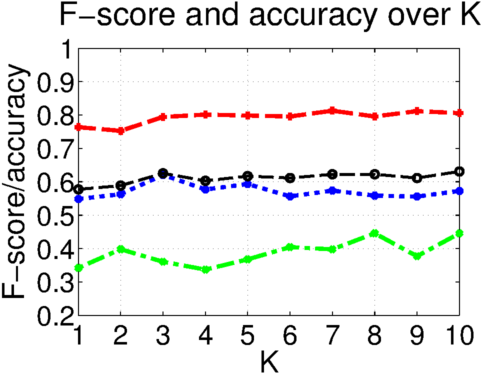
\includegraphics[width=0.3\textwidth]{tex/appendices/test/sflux105FP.png}
	\centering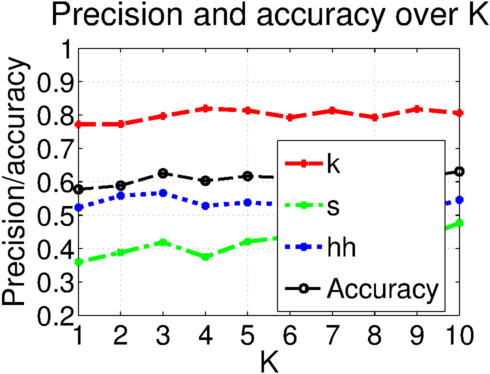
\includegraphics[width=0.3\textwidth]{tex/appendices/test/sflux105_P.png}
	\centering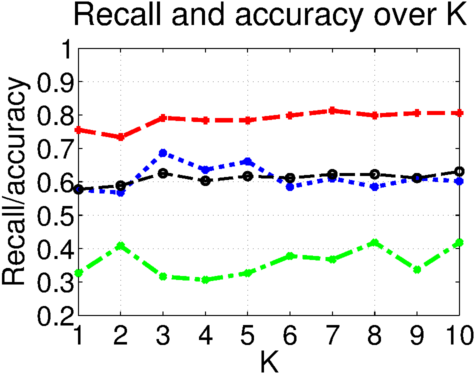
\includegraphics[width=0.3\textwidth]{tex/appendices/test/sflux105_R.png}
		
		\caption{Plots over K for Spectral Flux with 10ms windows and 5ms window skips}
\end{figure}
\begin{figure}


	\centering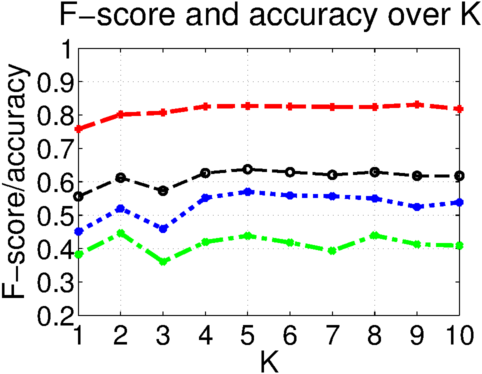
\includegraphics[width=0.3\textwidth]{tex/appendices/test/sflux52FP.png}
	\centering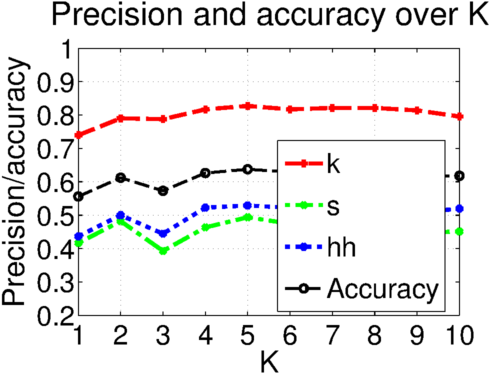
\includegraphics[width=0.3\textwidth]{tex/appendices/test/sflux52_P.png}
	\centering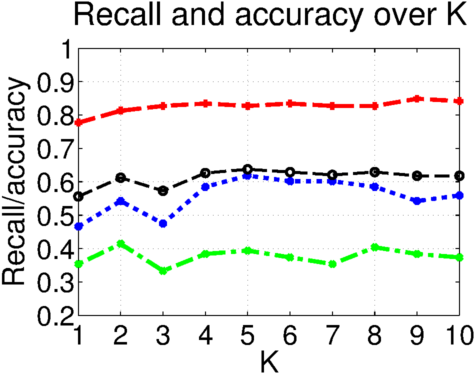
\includegraphics[width=0.3\textwidth]{tex/appendices/test/sflux52_R.png}
		
		\caption{Plots over K for Spectral Flux with 5ms windows and 2ms window skips}
\end{figure}

\begin{table}
\begin{subtable}[h]{0.45\textwidth}
\centering
\begin{tabular}{|c|c|c|c"c|}
\cline{2-5}
 \multicolumn{1}{c|}{} & \textbf{k}  & \textbf{s}  & \textbf{hh}  & Prec.\\ \hline
 \textbf{k} & \textcolor{red}{0.804} & 0.293 & 0.265 & 0.657\\ \hline
 \textbf{s} & 0.087 & \textcolor{red}{0.315} & 0.256 & 0.408\\ \hline
 \textbf{hh} & 0.087 & 0.391 & \textcolor{red}{0.479} & 0.523\\ \Xhline{2\arrayrulewidth}
 F & 0.723 & 0.356 & 0.500 & \textcolor{blue}{0.565}\\ \hline
\end{tabular}
\caption{$K=1$}
\end{subtable}
\hfill
\begin{subtable}[h]{0.45\textwidth}
\centering
\begin{tabular}{|c|c|c|c"c|}
\cline{2-5}
 \multicolumn{1}{c|}{} & \textbf{k}  & \textbf{s}  & \textbf{hh}  & Prec.\\ \hline
 \textbf{k} & \textcolor{red}{0.812} & 0.293 & 0.274 & 0.655\\ \hline
 \textbf{s} & 0.080 & \textcolor{red}{0.272} & 0.291 & 0.357\\ \hline
 \textbf{hh} & 0.080 & 0.435 & \textcolor{red}{0.436} & 0.481\\ \Xhline{2\arrayrulewidth}
 F & 0.725 & 0.309 & 0.457 & \textcolor{blue}{0.542}\\ \hline
\end{tabular}
\label{app:SF:2:worst}
\caption{$K=2$}
\end{subtable}
\hfill
\begin{subtable}[h]{0.45\textwidth}
\centering
\begin{tabular}{|c|c|c|c"c|}
\cline{2-5}
 \multicolumn{1}{c|}{} & \textbf{k}  & \textbf{s}  & \textbf{hh}  & Prec.\\ \hline
 \textbf{k} & \textcolor{red}{0.826} & 0.272 & 0.265 & 0.671\\ \hline
 \textbf{s} & 0.043 & \textcolor{red}{0.250} & 0.222 & 0.418\\ \hline
 \textbf{hh} & 0.043 & 0.478 & \textcolor{red}{0.513} & 0.492\\ \Xhline{2\arrayrulewidth}
 F & 0.740 & 0.313 & 0.502 & \textcolor{blue}{0.568}\\ \hline
\end{tabular}
\caption{$K=3$}
\end{subtable}
\hfill
\begin{subtable}[h]{0.45\textwidth}
\centering
\begin{tabular}{|c|c|c|c"c|}
\cline{2-5}
 \multicolumn{1}{c|}{} & \textbf{k}  & \textbf{s}  & \textbf{hh}  & Prec.\\ \hline
 \textbf{k} & \textcolor{red}{0.819} & 0.239 & 0.248 & 0.689\\ \hline
 \textbf{s} & 0.051 & \textcolor{red}{0.239} & 0.214 & 0.407\\ \hline
 \textbf{hh} & 0.051 & 0.522 & \textcolor{red}{0.538} & 0.488\\ \Xhline{2\arrayrulewidth}
 F & 0.748 & 0.301 & 0.512 & \textcolor{blue}{0.571}\\ \hline
\end{tabular}
\caption{$K=4$}
\end{subtable}
\hfill
\begin{subtable}[h]{0.45\textwidth}
\centering
\begin{tabular}{|c|c|c|c"c|}
\cline{2-5}
 \multicolumn{1}{c|}{} & \textbf{k}  & \textbf{s}  & \textbf{hh}  & Prec.\\ \hline
 \textbf{k} & \textcolor{red}{0.826} & 0.250 & 0.231 & 0.695\\ \hline
 \textbf{s} & 0.022 & \textcolor{red}{0.261} & 0.231 & 0.444\\ \hline
 \textbf{hh} & 0.022 & 0.489 & \textcolor{red}{0.538} & 0.488\\ \Xhline{2\arrayrulewidth}
 F & 0.755 & 0.329 & 0.512 & \textcolor{blue}{0.579}\\ \hline
\end{tabular}
\caption{$K=5$}
\end{subtable}
\hfill
\begin{subtable}[h]{0.45\textwidth}
\centering
\begin{tabular}{|c|c|c|c"c|}
\cline{2-5}
 \multicolumn{1}{c|}{} & \textbf{k}  & \textbf{s}  & \textbf{hh}  & Prec.\\ \hline
 \textbf{k} & \textcolor{red}{0.841} & 0.250 & 0.205 & 0.712\\ \hline
 \textbf{s} & 0.022 & \textcolor{red}{0.228} & 0.171 & 0.477\\ \hline
 \textbf{hh} & 0.022 & 0.522 & \textcolor{red}{0.624} & 0.521\\ \Xhline{2\arrayrulewidth}
 F & 0.771 & 0.309 & 0.568 & \textcolor{blue}{0.605}\\ \hline
\end{tabular}
\caption{$K=6$}
\end{subtable}
\hfill
\begin{subtable}[h]{0.45\textwidth}
\centering
\begin{tabular}{|c|c|c|c"c|}
\cline{2-5}
 \multicolumn{1}{c|}{} & \textbf{k}  & \textbf{s}  & \textbf{hh}  & Prec.\\ \hline
 \textbf{k} & \textcolor{red}{0.841} & 0.250 & 0.188 & 0.720\\ \hline
 \textbf{s} & 0.014 & \textcolor{red}{0.239} & 0.239 & 0.423\\ \hline
 \textbf{hh} & 0.014 & 0.511 & \textcolor{red}{0.573} & 0.500\\ \Xhline{2\arrayrulewidth}
 F & 0.776 & 0.306 & 0.534 & \textcolor{blue}{0.591}\\ \hline
\end{tabular}
\caption{$K=7$}
\end{subtable}
\hfill
\begin{subtable}[h]{0.45\textwidth}
\centering
\begin{tabular}{|c|c|c|c"c|}
\cline{2-5}
 \multicolumn{1}{c|}{} & \textbf{k}  & \textbf{s}  & \textbf{hh}  & Prec.\\ \hline
 \textbf{k} & \textcolor{red}{0.848} & 0.250 & 0.188 & 0.722\\ \hline
 \textbf{s} & 0.014 & \textcolor{red}{0.239} & 0.197 & 0.468\\ \hline
 \textbf{hh} & 0.014 & 0.511 & \textcolor{red}{0.615} & 0.522\\ \Xhline{2\arrayrulewidth}
 F & 0.780 & 0.317 & 0.565 & \textcolor{blue}{0.608}\\ \hline
\end{tabular}
\caption{$K=8$}
\end{subtable}
\hfill
\begin{subtable}[h]{0.45\textwidth}
\centering
\begin{tabular}{|c|c|c|c"c|}
\cline{2-5}
 \multicolumn{1}{c|}{} & \textbf{k}  & \textbf{s}  & \textbf{hh}  & Prec.\\ \hline
 \textbf{k} & \textcolor{red}{0.855} & 0.272 & 0.162 & 0.728\\ \hline
 \textbf{s} & 0.014 & \textcolor{red}{0.239} & 0.222 & 0.440\\ \hline
 \textbf{hh} & 0.014 & 0.489 & \textcolor{red}{0.615} & 0.533\\ \Xhline{2\arrayrulewidth}
 F & 0.787 & 0.310 & 0.571 & \textcolor{blue}{0.611}\\ \hline
\end{tabular}
\caption{$K=9$}
\end{subtable}
\hfill
\begin{subtable}[h]{0.45\textwidth}
\centering
\begin{tabular}{|c|c|c|c"c|}
\cline{2-5}
 \multicolumn{1}{c|}{} & \textbf{k}  & \textbf{s}  & \textbf{hh}  & Prec.\\ \hline
 \textbf{k} & \textcolor{red}{0.862} & 0.304 & 0.145 & 0.726\\ \hline
 \textbf{s} & 0.014 & \textcolor{red}{0.196} & 0.205 & 0.409\\ \hline
 \textbf{hh} & 0.014 & 0.500 & \textcolor{red}{0.650} & 0.547\\ \Xhline{2\arrayrulewidth}
 F & 0.788 & 0.265 & 0.594 & \textcolor{blue}{0.614}\\ \hline
\end{tabular}
\caption{$K=10$}
\end{subtable}
\hfill

\label{tlsflux2010}

\caption{tcsflux2010}

\end{table}

\newcolumntype{"}{@{\hskip\tabcolsep\vrule width 1pt\hskip\tabcolsep}}
\begin{table}

\begin{subtable}[h]{0.45\textwidth}
\centering
\scalebox{0.8}{
\begin{tabular}{|c|c|c|c|}\hline
 $K_1$ & $K_2$ & $X^2$ & p\\ \hline
 1 & 2 & 72.000 & 0.23040\\ \hline 
 1 & 3 & 72.000 & 0.23040\\ \hline 
 1 & 4 & 63.000 & 0.24255\\ \hline 
 1 & 5 & 63.000 & 0.24255\\ \hline 
 1 & 6 & 72.000 & 0.23040\\ \hline 
 1 & 7 & 63.000 & 0.24255\\ \hline 
 1 & 8 & 54.000 & 0.25605\\ \hline 
 1 & 9 & 72.000 & 0.23040\\ \hline 
 1 & 10 & 63.000 & 0.24255\\ \hline 
 2 & 3 & 72.000 & 0.23040\\ \hline 
 2 & 4 & 63.000 & 0.24255\\ \hline 
 2 & 5 & 63.000 & 0.24255\\ \hline 
 2 & 6 & 72.000 & 0.23040\\ \hline 
 2 & 7 & 63.000 & 0.24255\\ \hline 
 2 & 8 & 54.000 & 0.25605\\ \hline 
 2 & 9 & 72.000 & 0.23040\\ \hline 
 2 & 10 & 63.000 & 0.24255\\ \hline 
 3 & 4 & 63.000 & 0.24255\\ \hline 
 3 & 5 & 63.000 & 0.24255\\ \hline 
 3 & 6 & 72.000 & 0.23040\\ \hline 
 3 & 7 & 63.000 & 0.24255\\ \hline 
 3 & 8 & 54.000 & 0.25605\\ \hline 
 3 & 9 & 72.000 & 0.23040\\ \hline 
 3 & 10 & 63.000 & 0.24255\\ \hline 
 4 & 5 & 54.000 & 0.28935\\ \hline 
 4 & 6 & 63.000 & 0.24255\\ \hline 
 4 & 7 & 56.250 & 0.22185\\ \hline 
 4 & 8 & 49.500 & 0.19890\\ \hline 
 4 & 9 & 63.000 & 0.24255\\ \hline 
 4 & 10 & 54.000 & 0.28935\\ \hline 
 5 & 6 & 63.000 & 0.24255\\ \hline 
 5 & 7 & 56.250 & 0.22185\\ \hline 
 5 & 8 & 49.500 & 0.19890\\ \hline 
 5 & 9 & 63.000 & 0.24255\\ \hline 
 5 & 10 & 56.250 & 0.22185\\ \hline 
 6 & 7 & 63.000 & 0.24255\\ \hline
 6 & 8 & 54.000 & 0.25605\\ \hline 
 6 & 9 & 72.000 & 0.23040\\ \hline 
 6 & 10 & 63.000 & 0.24255\\ \hline 
 7 & 8 & 54.000 & 0.10125\\ \hline 
 7 & 9 & 63.000 & 0.24255\\ \hline 
 7 & 10 & 56.250 & 0.22185\\ \hline 
 8 & 9 & 54.000 & 0.25605\\ \hline 
 8 & 10 & 47.250 & 0.26685\\ \hline 
 9 & 10 & 63.000 & 0.24255\\ \hline 

\end{tabular}
}\label{xlsflux2010}
\caption{xcsflux2010}
\end{subtable}

\begin{subtable}[h]{0.45\textwidth}
\centering
\begin{tabular}{|c|c|c|}
\hline
Class & Amount & Percent\\ \hline
k & 461 & 32.93\\ \hline
undefined & 125 & 8.93\\ \hline
s & 307 & 21.93\\ \hline
\end{tabular}
\caption{Entire dataset after stripping short sounds}
\end{subtable}
\hfill
\begin{subtable}[h]{0.45\textwidth}
\centering
\begin{tabular}{|c|c|c|}
\hline
Class & Amount & Percent\\ \hline
k & 322 & 39.80\\ \hline
s & 214 & 26.45\\ \hline
hh & 273 & 33.75\\ \hline
\end{tabular}
\caption{Training dataset}
\end{subtable}
\hfill
\begin{subtable}[h]{0.45\textwidth}
\centering
\begin{tabular}{|c|c|c|}
\hline
Class & Amount & Percent\\ \hline
k & 138 & 39.77\\ \hline
s & 92 & 26.51\\ \hline
hh & 117 & 33.72\\ \hline
\end{tabular}
\caption{Testing dataset}
\end{subtable}
\hfill

\label{dlsflux2010}

\caption{dcsflux2010}

\end{table}

\newcolumntype{"}{@{\hskip\tabcolsep\vrule width 1pt\hskip\tabcolsep}}
\begin{table}
\begin{subtable}[h]{0.45\textwidth}
\centering
\begin{tabular}{|c|c|c|c"c|}
\cline{2-5}
 \multicolumn{1}{c|}{} & \textbf{k}  & \textbf{s}  & \textbf{hh}  & Prec.\\ \hline
 \textbf{k} & \textcolor{red}{0.755} & 0.235 & 0.068 & 0.772\\ \hline
 \textbf{s} & 0.108 & \textcolor{red}{0.327} & 0.356 & 0.360\\ \hline
 \textbf{hh} & 0.108 & 0.439 & \textcolor{red}{0.576} & 0.523\\ \Xhline{2\arrayrulewidth}
 F & 0.764 & 0.342 & 0.548 & \textcolor{blue}{0.577}\\ \hline
\end{tabular}
\caption{$K=1$}
\end{subtable}
\hfill
\begin{subtable}[h]{0.45\textwidth}
\centering
\begin{tabular}{|c|c|c|c"c|}
\cline{2-5}
 \multicolumn{1}{c|}{} & \textbf{k}  & \textbf{s}  & \textbf{hh}  & Prec.\\ \hline
 \textbf{k} & \textcolor{red}{0.734} & 0.214 & 0.076 & 0.773\\ \hline
 \textbf{s} & 0.151 & \textcolor{red}{0.408} & 0.356 & 0.388\\ \hline
 \textbf{hh} & 0.151 & 0.378 & \textcolor{red}{0.568} & 0.558\\ \Xhline{2\arrayrulewidth}
 F & 0.753 & 0.398 & 0.563 & \textcolor{blue}{0.589}\\ \hline
\end{tabular}
\caption{$K=2$}
\end{subtable}
\hfill
\begin{subtable}[h]{0.45\textwidth}
\centering
\begin{tabular}{|c|c|c|c"c|}
\cline{2-5}
 \multicolumn{1}{c|}{} & \textbf{k}  & \textbf{s}  & \textbf{hh}  & Prec.\\ \hline
 \textbf{k} & \textcolor{red}{0.791} & 0.204 & 0.068 & 0.797\\ \hline
 \textbf{s} & 0.101 & \textcolor{red}{0.316} & 0.246 & 0.419\\ \hline
 \textbf{hh} & 0.101 & 0.480 & \textcolor{red}{0.686} & 0.566\\ \Xhline{2\arrayrulewidth}
 F & 0.794 & 0.360 & 0.621 & \textcolor{blue}{0.625}\\ \hline
\end{tabular}
\caption{$K=3$}
\end{subtable}
\hfill
\begin{subtable}[h]{0.45\textwidth}
\centering
\begin{tabular}{|c|c|c|c"c|}
\cline{2-5}
 \multicolumn{1}{c|}{} & \textbf{k}  & \textbf{s}  & \textbf{hh}  & Prec.\\ \hline
 \textbf{k} & \textcolor{red}{0.784} & 0.173 & 0.059 & 0.820\\ \hline
 \textbf{s} & 0.101 & \textcolor{red}{0.306} & 0.305 & 0.375\\ \hline
 \textbf{hh} & 0.101 & 0.520 & \textcolor{red}{0.636} & 0.528\\ \Xhline{2\arrayrulewidth}
 F & 0.801 & 0.337 & 0.577 & \textcolor{blue}{0.603}\\ \hline
\end{tabular}
\caption{$K=4$}
\end{subtable}
\hfill
\begin{subtable}[h]{0.45\textwidth}
\centering
\begin{tabular}{|c|c|c|c"c|}
\cline{2-5}
 \multicolumn{1}{c|}{} & \textbf{k}  & \textbf{s}  & \textbf{hh}  & Prec.\\ \hline
 \textbf{k} & \textcolor{red}{0.784} & 0.163 & 0.076 & 0.813\\ \hline
 \textbf{s} & 0.094 & \textcolor{red}{0.327} & 0.263 & 0.421\\ \hline
 \textbf{hh} & 0.094 & 0.510 & \textcolor{red}{0.661} & 0.538\\ \Xhline{2\arrayrulewidth}
 F & 0.799 & 0.368 & 0.593 & \textcolor{blue}{0.617}\\ \hline
\end{tabular}
\caption{$K=5$}
\end{subtable}
\hfill
\begin{subtable}[h]{0.45\textwidth}
\centering
\begin{tabular}{|c|c|c|c"c|}
\cline{2-5}
 \multicolumn{1}{c|}{} & \textbf{k}  & \textbf{s}  & \textbf{hh}  & Prec.\\ \hline
 \textbf{k} & \textcolor{red}{0.799} & 0.163 & 0.110 & 0.793\\ \hline
 \textbf{s} & 0.086 & \textcolor{red}{0.378} & 0.305 & 0.435\\ \hline
 \textbf{hh} & 0.086 & 0.459 & \textcolor{red}{0.585} & 0.531\\ \Xhline{2\arrayrulewidth}
 F & 0.796 & 0.404 & 0.556 & \textcolor{blue}{0.611}\\ \hline
\end{tabular}
\caption{$K=6$}
\end{subtable}
\hfill
\begin{subtable}[h]{0.45\textwidth}
\centering
\begin{tabular}{|c|c|c|c"c|}
\cline{2-5}
 \multicolumn{1}{c|}{} & \textbf{k}  & \textbf{s}  & \textbf{hh}  & Prec.\\ \hline
 \textbf{k} & \textcolor{red}{0.813} & 0.163 & 0.085 & 0.813\\ \hline
 \textbf{s} & 0.079 & \textcolor{red}{0.367} & 0.305 & 0.434\\ \hline
 \textbf{hh} & 0.079 & 0.469 & \textcolor{red}{0.610} & 0.541\\ \Xhline{2\arrayrulewidth}
 F & 0.813 & 0.398 & 0.574 & \textcolor{blue}{0.623}\\ \hline
\end{tabular}
\caption{$K=7$}
\end{subtable}
\hfill
\begin{subtable}[h]{0.45\textwidth}
\centering
\begin{tabular}{|c|c|c|c"c|}
\cline{2-5}
 \multicolumn{1}{c|}{} & \textbf{k}  & \textbf{s}  & \textbf{hh}  & Prec.\\ \hline
 \textbf{k} & \textcolor{red}{0.799} & 0.163 & 0.110 & 0.793\\ \hline
 \textbf{s} & 0.065 & \textcolor{red}{0.418} & 0.305 & 0.477\\ \hline
 \textbf{hh} & 0.065 & 0.418 & \textcolor{red}{0.585} & 0.535\\ \Xhline{2\arrayrulewidth}
 F & 0.796 & 0.446 & 0.559 & \textcolor{blue}{0.623}\\ \hline
\end{tabular}
\caption{$K=8$}
\end{subtable}
\hfill
\begin{subtable}[h]{0.45\textwidth}
\centering
\begin{tabular}{|c|c|c|c"c|}
\cline{2-5}
 \multicolumn{1}{c|}{} & \textbf{k}  & \textbf{s}  & \textbf{hh}  & Prec.\\ \hline
 \textbf{k} & \textcolor{red}{0.806} & 0.163 & 0.076 & 0.818\\ \hline
 \textbf{s} & 0.050 & \textcolor{red}{0.337} & 0.314 & 0.429\\ \hline
 \textbf{hh} & 0.050 & 0.500 & \textcolor{red}{0.610} & 0.511\\ \Xhline{2\arrayrulewidth}
 F & 0.812 & 0.377 & 0.556 & \textcolor{blue}{0.611}\\ \hline
\end{tabular}
\caption{$K=9$}
\end{subtable}
\hfill
\begin{subtable}[h]{0.45\textwidth}
\centering
\begin{tabular}{|c|c|c|c"c|}
\cline{2-5}
 \multicolumn{1}{c|}{} & \textbf{k}  & \textbf{s}  & \textbf{hh}  & Prec.\\ \hline
 \textbf{k} & \textcolor{red}{0.806} & 0.173 & 0.085 & 0.806\\ \hline
 \textbf{s} & 0.058 & \textcolor{red}{0.418} & 0.314 & 0.477\\ \hline
 \textbf{hh} & 0.058 & 0.408 & \textcolor{red}{0.602} & 0.546\\ \Xhline{2\arrayrulewidth}
 F & 0.806 & 0.446 & 0.573 & \textcolor{blue}{0.631}\\ \hline
\end{tabular}
\caption{$K=10$}
\end{subtable}
\hfill

\label{tlsflux105}

\caption{tcsflux105}

\end{table}

\newcolumntype{"}{@{\hskip\tabcolsep\vrule width 1pt\hskip\tabcolsep}}
\begin{table}

\begin{subtable}[h]{0.45\textwidth}
\centering
\scalebox{0.8}{
\begin{tabular}{|c|c|c|c|}\hline
 $K_1$ & $K_2$ & $X^2$ & p\\ \hline
 1 & 2 & 63.000 & 0.24255\\ \hline 
 1 & 3 & 72.000 & 0.23040\\ \hline 
 1 & 4 & 72.000 & 0.23040\\ \hline 
 1 & 5 & 72.000 & 0.23040\\ \hline 
 1 & 6 & 63.000 & 0.24255\\ \hline 
 1 & 7 & 63.000 & 0.24255\\ \hline 
 1 & 8 & 63.000 & 0.24255\\ \hline 
 1 & 9 & 72.000 & 0.23040\\ \hline 
 1 & 10 & 72.000 & 0.23040\\ \hline 
 2 & 3 & 63.000 & 0.24255\\ \hline 
 2 & 4 & 63.000 & 0.24255\\ \hline 
 2 & 5 & 63.000 & 0.24255\\ \hline 
 2 & 6 & 56.250 & 0.22185\\ \hline 
 2 & 7 & 54.000 & 0.28935\\ \hline 
 2 & 8 & 54.000 & 0.28935\\ \hline 
 2 & 9 & 63.000 & 0.24255\\ \hline 
 2 & 10 & 63.000 & 0.24255\\ \hline 
 3 & 4 & 72.000 & 0.23040\\ \hline 
 3 & 5 & 72.000 & 0.23040\\ \hline 
 3 & 6 & 63.000 & 0.24255\\ \hline 
 3 & 7 & 63.000 & 0.24255\\ \hline 
 3 & 8 & 63.000 & 0.24255\\ \hline 
 3 & 9 & 72.000 & 0.23040\\ \hline 
 3 & 10 & 72.000 & 0.23040\\ \hline 
 4 & 5 & 72.000 & 0.23040\\ \hline 
 4 & 6 & 63.000 & 0.24255\\ \hline 
 4 & 7 & 63.000 & 0.24255\\ \hline 
 4 & 8 & 63.000 & 0.24255\\ \hline 
 4 & 9 & 72.000 & 0.23040\\ \hline 
 4 & 10 & 72.000 & 0.23040\\ \hline 
 5 & 6 & 63.000 & 0.24255\\ \hline 
 5 & 7 & 63.000 & 0.24255\\ \hline 
 5 & 8 & 63.000 & 0.24255\\ \hline 
 5 & 9 & 72.000 & 0.23040\\ \hline 
 5 & 10 & 72.000 & 0.23040\\ \hline 
 6 & 7 & 54.000 & 0.28935\\ \hline 
 6 & 8 & 54.000 & 0.28935\\ \hline 
 6 & 9 & 63.000 & 0.24255\\ \hline 
 6 & 10 & 63.000 & 0.24255\\ \hline 
 7 & 8 & 56.250 & 0.22185\\ \hline 
 7 & 9 & 63.000 & 0.24255\\ \hline 
 7 & 10 & 63.000 & 0.24255\\ \hline 
 8 & 9 & 63.000 & 0.24255\\ \hline 
 8 & 10 & 63.000 & 0.24255\\ \hline 
 9 & 10 & 72.000 & 0.23040\\ \hline 

\end{tabular}
}\label{xlsflux105}
\caption{xcsflux105}
\end{subtable}

\begin{subtable}[h]{0.45\textwidth}
\centering
\begin{tabular}{|c|c|c|}
\hline
Class & Amount & Percent\\ \hline
noise & 138 & 9.47\\ \hline
k & 466 & 31.98\\ \hline
undefined & 130 & 8.92\\ \hline
\end{tabular}
\caption{Entire dataset after stripping short sounds}
\end{subtable}
\hfill
\begin{subtable}[h]{0.45\textwidth}
\centering
\begin{tabular}{|c|c|c|}
\hline
Class & Amount & Percent\\ \hline
k & 326 & 39.23\\ \hline
s & 229 & 27.56\\ \hline
hh & 276 & 33.21\\ \hline
\end{tabular}
\caption{Training dataset}
\end{subtable}
\hfill
\begin{subtable}[h]{0.45\textwidth}
\centering
\begin{tabular}{|c|c|c|}
\hline
Class & Amount & Percent\\ \hline
k & 139 & 39.15\\ \hline
s & 98 & 27.61\\ \hline
hh & 118 & 33.24\\ \hline
\end{tabular}
\caption{Testing dataset}
\end{subtable}
\hfill

\label{dlsflux105}

\caption{dcsflux105}

\end{table}

\newcolumntype{"}{@{\hskip\tabcolsep\vrule width 1pt\hskip\tabcolsep}}
\begin{table}
\begin{subtable}[h]{0.45\textwidth}
\centering
\begin{tabular}{|c|c|c|c"c|}
\cline{2-5}
 \multicolumn{1}{c|}{} & \textbf{k}  & \textbf{s}  & \textbf{hh}  & Prec.\\ \hline
 \textbf{k} & \textcolor{red}{0.777} & 0.162 & 0.186 & 0.740\\ \hline
 \textbf{s} & 0.058 & \textcolor{red}{0.354} & 0.347 & 0.417\\ \hline
 \textbf{hh} & 0.058 & 0.485 & \textcolor{red}{0.466} & 0.437\\ \Xhline{2\arrayrulewidth}
 F & 0.758 & 0.383 & 0.451 & \textcolor{blue}{0.556}\\ \hline
\end{tabular}
\caption{$K=1$}
\end{subtable}
\hfill
\begin{subtable}[h]{0.45\textwidth}
\centering
\begin{tabular}{|c|c|c|c"c|}
\cline{2-5}
 \multicolumn{1}{c|}{} & \textbf{k}  & \textbf{s}  & \textbf{hh}  & Prec.\\ \hline
 \textbf{k} & \textcolor{red}{0.813} & 0.141 & 0.136 & 0.790\\ \hline
 \textbf{s} & 0.043 & \textcolor{red}{0.414} & 0.322 & 0.482\\ \hline
 \textbf{hh} & 0.043 & 0.444 & \textcolor{red}{0.542} & 0.500\\ \Xhline{2\arrayrulewidth}
 F & 0.801 & 0.446 & 0.520 & \textcolor{blue}{0.612}\\ \hline
\end{tabular}
\caption{$K=2$}
\end{subtable}
\hfill
\begin{subtable}[h]{0.45\textwidth}
\centering
\begin{tabular}{|c|c|c|c"c|}
\cline{2-5}
 \multicolumn{1}{c|}{} & \textbf{k}  & \textbf{s}  & \textbf{hh}  & Prec.\\ \hline
 \textbf{k} & \textcolor{red}{0.827} & 0.131 & 0.153 & 0.788\\ \hline
 \textbf{s} & 0.050 & \textcolor{red}{0.333} & 0.373 & 0.393\\ \hline
 \textbf{hh} & 0.050 & 0.535 & \textcolor{red}{0.475} & 0.444\\ \Xhline{2\arrayrulewidth}
 F & 0.807 & 0.361 & 0.459 & \textcolor{blue}{0.573}\\ \hline
\end{tabular}
\caption{$K=3$}
\end{subtable}
\hfill
\begin{subtable}[h]{0.45\textwidth}
\centering
\begin{tabular}{|c|c|c|c"c|}
\cline{2-5}
 \multicolumn{1}{c|}{} & \textbf{k}  & \textbf{s}  & \textbf{hh}  & Prec.\\ \hline
 \textbf{k} & \textcolor{red}{0.835} & 0.131 & 0.110 & 0.817\\ \hline
 \textbf{s} & 0.058 & \textcolor{red}{0.384} & 0.305 & 0.463\\ \hline
 \textbf{hh} & 0.058 & 0.485 & \textcolor{red}{0.585} & 0.523\\ \Xhline{2\arrayrulewidth}
 F & 0.826 & 0.420 & 0.552 & \textcolor{blue}{0.626}\\ \hline
\end{tabular}
\caption{$K=4$}
\end{subtable}
\hfill
\begin{subtable}[h]{0.45\textwidth}
\centering
\begin{tabular}{|c|c|c|c"c|}
\cline{2-5}
 \multicolumn{1}{c|}{} & \textbf{k}  & \textbf{s}  & \textbf{hh}  & Prec.\\ \hline
 \textbf{k} & \textcolor{red}{0.827} & 0.121 & 0.102 & 0.827\\ \hline
 \textbf{s} & 0.050 & \textcolor{red}{0.394} & 0.280 & 0.494\\ \hline
 \textbf{hh} & 0.050 & 0.485 & \textcolor{red}{0.619} & 0.529\\ \Xhline{2\arrayrulewidth}
 F & 0.827 & 0.438 & 0.570 & \textcolor{blue}{0.638}\\ \hline
\end{tabular}
\label{app:SF:5:best}
\caption{$K=5$}
\end{subtable}
\hfill
\begin{subtable}[h]{0.45\textwidth}
\centering
\begin{tabular}{|c|c|c|c"c|}
\cline{2-5}
 \multicolumn{1}{c|}{} & \textbf{k}  & \textbf{s}  & \textbf{hh}  & Prec.\\ \hline
 \textbf{k} & \textcolor{red}{0.835} & 0.141 & 0.102 & 0.817\\ \hline
 \textbf{s} & 0.043 & \textcolor{red}{0.374} & 0.297 & 0.474\\ \hline
 \textbf{hh} & 0.043 & 0.485 & \textcolor{red}{0.602} & 0.522\\ \Xhline{2\arrayrulewidth}
 F & 0.826 & 0.418 & 0.559 & \textcolor{blue}{0.629}\\ \hline
\end{tabular}
\caption{$K=6$}
\end{subtable}
\hfill
\begin{subtable}[h]{0.45\textwidth}
\centering
\begin{tabular}{|c|c|c|c"c|}
\cline{2-5}
 \multicolumn{1}{c|}{} & \textbf{k}  & \textbf{s}  & \textbf{hh}  & Prec.\\ \hline
 \textbf{k} & \textcolor{red}{0.827} & 0.141 & 0.093 & 0.821\\ \hline
 \textbf{s} & 0.058 & \textcolor{red}{0.354} & 0.305 & 0.443\\ \hline
 \textbf{hh} & 0.058 & 0.505 & \textcolor{red}{0.602} & 0.518\\ \Xhline{2\arrayrulewidth}
 F & 0.824 & 0.393 & 0.557 & \textcolor{blue}{0.621}\\ \hline
\end{tabular}
\caption{$K=7$}
\end{subtable}
\hfill
\begin{subtable}[h]{0.45\textwidth}
\centering
\begin{tabular}{|c|c|c|c"c|}
\cline{2-5}
 \multicolumn{1}{c|}{} & \textbf{k}  & \textbf{s}  & \textbf{hh}  & Prec.\\ \hline
 \textbf{k} & \textcolor{red}{0.827} & 0.131 & 0.102 & 0.821\\ \hline
 \textbf{s} & 0.043 & \textcolor{red}{0.404} & 0.314 & 0.482\\ \hline
 \textbf{hh} & 0.043 & 0.465 & \textcolor{red}{0.585} & 0.519\\ \Xhline{2\arrayrulewidth}
 F & 0.824 & 0.440 & 0.550 & \textcolor{blue}{0.629}\\ \hline
\end{tabular}
\caption{$K=8$}
\end{subtable}
\hfill
\begin{subtable}[h]{0.45\textwidth}
\centering
\begin{tabular}{|c|c|c|c"c|}
\cline{2-5}
 \multicolumn{1}{c|}{} & \textbf{k}  & \textbf{s}  & \textbf{hh}  & Prec.\\ \hline
 \textbf{k} & \textcolor{red}{0.849} & 0.141 & 0.110 & 0.814\\ \hline
 \textbf{s} & 0.043 & \textcolor{red}{0.384} & 0.347 & 0.447\\ \hline
 \textbf{hh} & 0.043 & 0.475 & \textcolor{red}{0.542} & 0.508\\ \Xhline{2\arrayrulewidth}
 F & 0.831 & 0.413 & 0.525 & \textcolor{blue}{0.618}\\ \hline
\end{tabular}
\caption{$K=9$}
\end{subtable}
\hfill
\begin{subtable}[h]{0.45\textwidth}
\centering
\begin{tabular}{|c|c|c|c"c|}
\cline{2-5}
 \multicolumn{1}{c|}{} & \textbf{k}  & \textbf{s}  & \textbf{hh}  & Prec.\\ \hline
 \textbf{k} & \textcolor{red}{0.842} & 0.162 & 0.119 & 0.796\\ \hline
 \textbf{s} & 0.050 & \textcolor{red}{0.374} & 0.322 & 0.451\\ \hline
 \textbf{hh} & 0.050 & 0.465 & \textcolor{red}{0.559} & 0.520\\ \Xhline{2\arrayrulewidth}
 F & 0.818 & 0.409 & 0.539 & \textcolor{blue}{0.618}\\ \hline
\end{tabular}
\caption{$K=10$}
\end{subtable}
\hfill

\label{tlsflux52}

\caption{tcsflux52}

\end{table}

\newcolumntype{"}{@{\hskip\tabcolsep\vrule width 1pt\hskip\tabcolsep}}
\begin{table}

\begin{subtable}[h]{0.45\textwidth}
\centering
\scalebox{0.8}{
\begin{tabular}{|c|c|c|c|}\hline
 $K_1$ & $K_2$ & $X^2$ & p\\ \hline
 1 & 2 & 72.000 & 0.23040\\ \hline 
 1 & 3 & 72.000 & 0.23040\\ \hline 
 1 & 4 & 63.000 & 0.24255\\ \hline 
 1 & 5 & 63.000 & 0.24255\\ \hline 
 1 & 6 & 72.000 & 0.23040\\ \hline 
 1 & 7 & 72.000 & 0.23040\\ \hline 
 1 & 8 & 72.000 & 0.23040\\ \hline 
 1 & 9 & 72.000 & 0.23040\\ \hline 
 1 & 10 & 72.000 & 0.23040\\ \hline 
 2 & 3 & 72.000 & 0.23040\\ \hline 
 2 & 4 & 63.000 & 0.24255\\ \hline 
 2 & 5 & 63.000 & 0.24255\\ \hline 
 2 & 6 & 72.000 & 0.23040\\ \hline 
 2 & 7 & 72.000 & 0.23040\\ \hline 
 2 & 8 & 72.000 & 0.23040\\ \hline 
 2 & 9 & 72.000 & 0.23040\\ \hline 
 2 & 10 & 72.000 & 0.23040\\ \hline 
 3 & 4 & 63.000 & 0.24255\\ \hline 
 3 & 5 & 63.000 & 0.24255\\ \hline 
 3 & 6 & 72.000 & 0.23040\\ \hline 
 3 & 7 & 72.000 & 0.23040\\ \hline 
 3 & 8 & 72.000 & 0.23040\\ \hline 
 3 & 9 & 72.000 & 0.23040\\ \hline 
 3 & 10 & 72.000 & 0.23040\\ \hline 
 4 & 5 & 63.000 & 0.08640\\ \hline 
 4 & 6 & 63.000 & 0.24255\\ \hline 
 4 & 7 & 63.000 & 0.24255\\ \hline 
 4 & 8 & 63.000 & 0.24255\\ \hline 
 4 & 9 & 63.000 & 0.24255\\ \hline 
 4 & 10 & 63.000 & 0.24255\\ \hline 
 5 & 6 & 63.000 & 0.24255\\ \hline 
 5 & 7 & 63.000 & 0.24255\\ \hline 
 5 & 8 & 63.000 & 0.24255\\ \hline 
 5 & 9 & 63.000 & 0.24255\\ \hline 
 5 & 10 & 63.000 & 0.24255\\ \hline 
 6 & 7 & 72.000 & 0.23040\\ \hline 
 6 & 8 & 72.000 & 0.23040\\ \hline 
 6 & 9 & 72.000 & 0.23040\\ \hline 
 6 & 10 & 72.000 & 0.23040\\ \hline 
 7 & 8 & 72.000 & 0.23040\\ \hline 
 7 & 9 & 72.000 & 0.23040\\ \hline 
 7 & 10 & 72.000 & 0.23040\\ \hline 
 8 & 9 & 72.000 & 0.23040\\ \hline 
 8 & 10 & 72.000 & 0.23040\\ \hline 
 9 & 10 & 72.000 & 0.23040\\ \hline 

\end{tabular}
}\label{xlsflux52}
\caption{xcsflux52}
\end{subtable}

\begin{subtable}[h]{0.45\textwidth}
\centering
\begin{tabular}{|c|c|c|}
\hline
Class & Amount & Percent\\ \hline
noise & 148 & 10.07\\ \hline
k & 466 & 31.70\\ \hline
undefined & 130 & 8.84\\ \hline
\end{tabular}
\caption{Entire dataset after stripping short sounds}
\end{subtable}
\hfill
\begin{subtable}[h]{0.45\textwidth}
\centering
\begin{tabular}{|c|c|c|}
\hline
Class & Amount & Percent\\ \hline
k & 326 & 39.14\\ \hline
s & 231 & 27.73\\ \hline
hh & 276 & 33.13\\ \hline
\end{tabular}
\caption{Training dataset}
\end{subtable}
\hfill
\begin{subtable}[h]{0.45\textwidth}
\centering
\begin{tabular}{|c|c|c|}
\hline
Class & Amount & Percent\\ \hline
k & 139 & 39.04\\ \hline
s & 99 & 27.81\\ \hline
hh & 118 & 33.15\\ \hline
\end{tabular}
\caption{Testing dataset}
\end{subtable}
\hfill

\label{dlsflux52}

\caption{dcsflux52}

\end{table}
